\documentclass[a4paper, 12pt]{article}%тип документа

%отступы
\usepackage[left=1.5cm,right=1cm,top=2cm,bottom=3cm,bindingoffset=0cm]{geometry}
\setlength{\parindent}{5ex}

%Русский язык
\usepackage[T2A]{fontenc} %кодировка
\usepackage[utf8]{inputenc} %кодировка исходного кода
\usepackage[english,russian]{babel} %локализация и переносы

%Вставка картинок
\usepackage{graphicx}
\graphicspath{{pictures/}}
\DeclareGraphicsExtensions{.pdf,.png,.jpg,}
\usepackage{wrapfig}

%Графики
\usepackage{pgfplots}
\pgfplotsset{compat=1.9}

%Математика
\usepackage{amsmath, amsfonts, amssymb, amsthm, mathtools}

%Таблицы
\usepackage{longtable} 
\usepackage{float}

%Римские цифры
\newcommand{\RomanNumeralCaps}[1]{\uppercase\expandafter{\romannumeral#1}}

\usepackage{multirow}


\begin{document}
	\begin{titlepage}
		\begin{center}
			\textsc{Федеральное государственное автономное образовательное учреждение высшего образования«Московский физико-технический институт (национальный исследовательский университет)»\\[5mm]
			}
			
			\vfill
			
			\textbf{Отчёт по лабораторной работе 5.2.2\\[3mm]
				Изучение спектров атома водорода и молекул йода
				\\[50mm]
			}
			
		\end{center}
		
		\hfill
		\begin{minipage}{.5\textwidth}
			Выполнил студент:\\[2mm]
			Сериков Василий Романович\\[2mm]
			группа: Б03-102\\[5mm]
			
		\end{minipage}
		\vfill
		\begin{center}
			Москва, 2023 г.
		\end{center}
		
	\end{titlepage}
	
	\newpage
	\setcounter{page}{2}
	\textbf{Аннотация}\\
	
	\textbf{Цель работы: }\\
	
	Исследовать сериальные закономерности в оптическом спектре водорода. Исследовать поглощения паров йода в видимой области.\\
	
	\textbf{Теория}\\  
	
	Атом водорода является простейшей квантовой системой, для которой уравнение Шредингера может быть решено точно. Это также верно для водородоподобных атомов, то есть атомов с одним электроном на внешней оболочке. Из решения уравнения Шредингера следует, что внешний электрон в таких атомах обладает дискретным энергетическим спектром:  
	\begin{equation}
		E_n = - \frac{m_e (Z e^2)^2}{2\hbar^2}\frac{1}{n^2},
	\end{equation}
	где $n$ есть номер энергетического уровня, $Z$ есть зарядовое число ядра рассматриваемого атома, которое в случае атома водорода равно 1.\\
	При переходе электрона с $n$-го на $m$-й уровень излучается фотон с энергией
	\begin{equation}
		E_\gamma = E_n - E_m = \frac{m_ee^2}{2\hbar^2}Z^2\left(\frac{1}{m^2} - \frac{1}{n^2}\right).
	\end{equation}
	Длина волны  соответствующего излучения $\lambda_{n,m}$ связана с номерами уровней следующим соотношением:
	\begin{equation}
		\label{eq:Ry}
		\lambda_{n,m}^{-1} =\frac{m_ee^2}{4\pi\hbar^3c}Z^2\left(\frac{1}{m^2}-\frac{1}{n^2}\right) = \text{Ry} Z^2 \left(\frac{1}{m^2}-\frac{1}{n^2}\right),
	\end{equation}
	где $\text{Ry} = \frac{m_ee^2}{4\pi\hbar^3c}$ есть постоянная Ридберга.
	
	В данной работе будет исследоваться серия Бальмера атома водорода, в которой электроны совершают переходы с некоторого уровня $n$ на уровень $m = 2$.\\

	В первом приближении энергия молекулы может быть представлена в виде:
	\begin{equation}
		E=E_e+E_o+E_r,
	\end{equation}
	где $E_e$ есть энергия электронных уровней, $E_o$ есть энергия колебательных уровней, $E_r$ есть энергия вращательных уровней.
	
	В настоящей работе рассматриваются оптические переходы, то есть переходы, связанные с излучением фотонов в видимом диапазоне длин волн. Они соответствуют переходам между различными электронными состояниями. При этом также происходят изменения вращательного и колебательного состояний, однако в реальности ввиду малости характерных энергий вращательные переходы не наблюдаемы.
	
	Более конкретно, изучаются переходы из колебательного состояния с номером $n_1$ основного электронного уровня с энергией $E_1$ в колебательное состояние с номером $n_2$ на электронный уровень с энергией $E_2$. Энергия таких переходов описывается формулой:
	\begin{equation}
		h \nu_{n_1,n_2}=(E_2-E_1)+h\nu_2(n_2+\dfrac{1}{2})-h \nu_1(n_1+\dfrac{1}{2}),
	\end{equation}
	где $\nu_1$ и $\nu_2$ суть энергии колебательных квантов на электронных уровнях с энергиями $E_1$ и $E_2$.
	
	При достаточно больших квантовых числах $n_1$ и $n_2$ колебательные уровни переходят в непрерывный спектр, что соответствует диссоциации молекулы. Наименьшая энергия, которую нужно сообщить молекуле в нижайшем колебательном состоянии, чтобы она диссоциировала, называется энергией диссоциации.
	
	В данной работе определяются энергии диссоциации на первых двух электронных уровнях.
	
	 Изучение молекулярного спектра йода в данной работе проводиться с помощью источника сплошного спектра - лампы накаливания. Кристаллы йода подогреваются в результате этого частично возгоняются, образуя пары. Спектрометр позволяет визуально наблюдать линии поглощения молекул йода на фоне сплошного спектра излучения лампы.\\
	
	\textbf{Экспериментальная установка: }\\
	
	Для измерения длин волн спектральных линий в работе используется стеклянно-призменный монохроматор-спектрометр УМ-2, предназначенный для спектральных исследований в диапазоне от 0,38 до 1,00 мкм
	
	\begin{figure}[H]
		\centering
		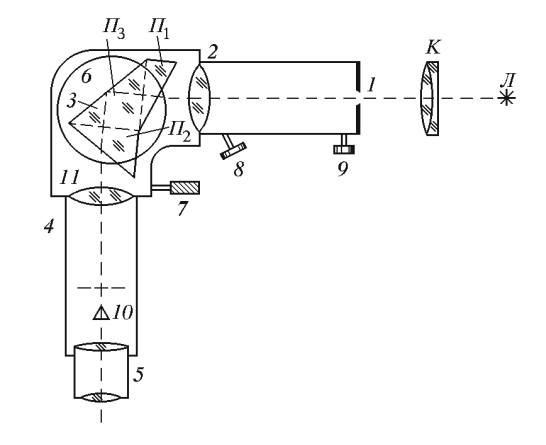
\includegraphics[width=0.6\linewidth]{ust}
		\caption{Схема установки}
	\end{figure}
	
	\newpage

	\textbf{Ход работы: }\\
	
	\begin{enumerate}
		
		\item Проградуируем спектрометр по спектру неона. Расположение спектральных линий неона и длины волн приведем на Рис 2. Полученные данные занесем в таблицу 1.
		
		\begin{figure}[H]
			\center{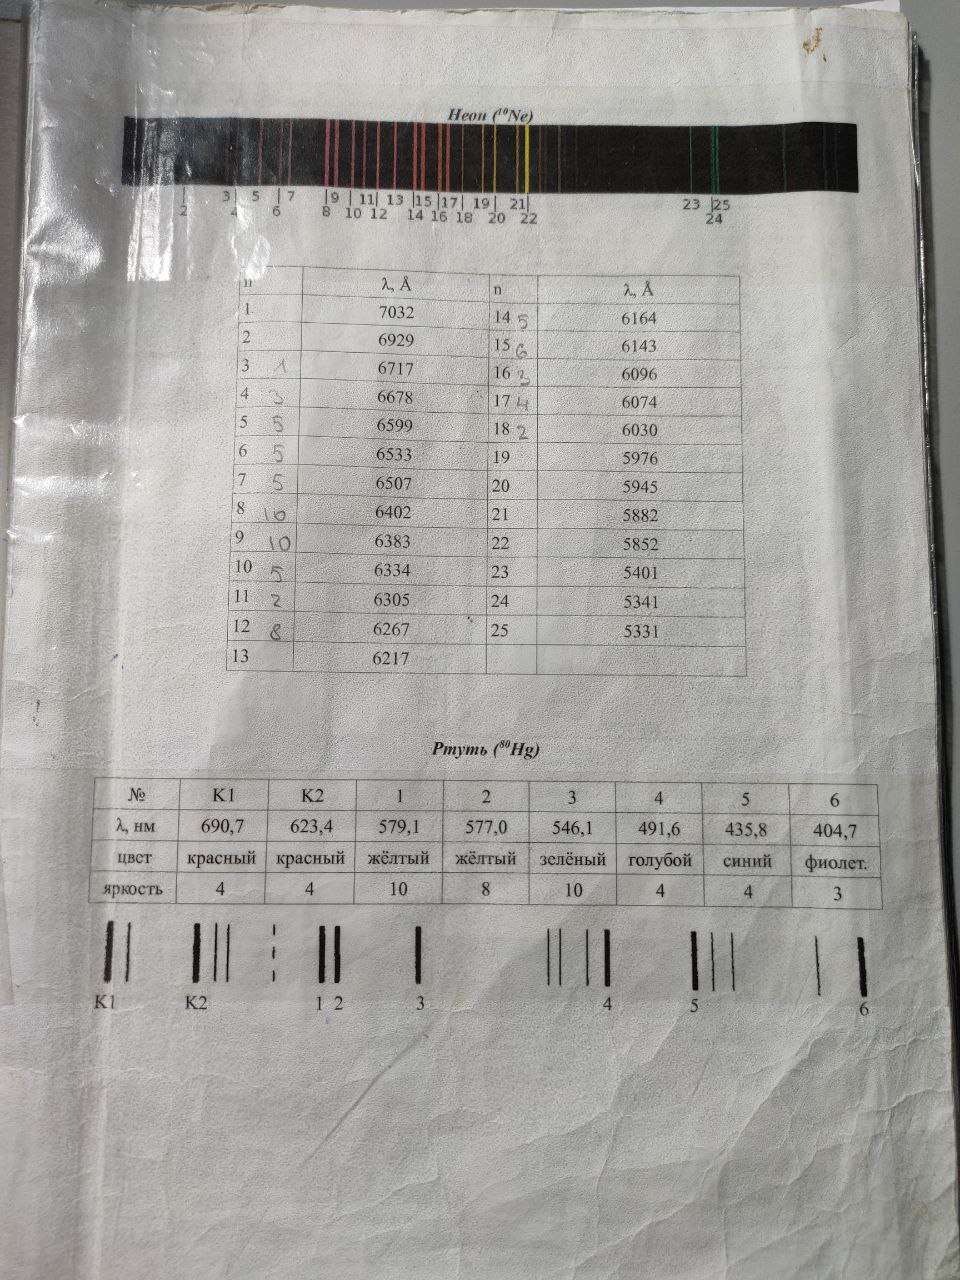
\includegraphics[scale=0.45]{neon}}
			\caption{Расположение спектральных линий неона и длины волн линий неона. Расположение спектральных линий ртути, длины волн основных спектральных линий ртути.}
		\end{figure}
		
		\begin{longtable}{|c|c|c|c|c|c|c|c|c|c|c|c|c|c|}
			\hline
			№ & 1 & 2 & 3 & 4 & 5 & 6 & 7 & 8 & 9 & 10 & 11 & 12 & 13 \\ \hline
			$\theta, {}^\circ$ & 2632 & 2600 & 2538 & 2524 & 2496 & 2476 & 2464 & 2418 & 2414 & 2398 & 2388 & 2368 & 2350 \\ \hline
			
			\hline 
			
			№ & 14 & 15 & 16 & 17 & 18 & 19 & 20 & 21 & 22 & 23 & 24 & 25 &  \\ \hline
			$\theta, {}^\circ$ & 2328 & 2314 & 2300 & 2290 & 2268 & 2240 & 2224 & 2198 & 2182 & 1914 & 1872 & 1868 &  \\ \hline
			
			\caption{Значения угла барабана при различных спектральных линиях неона. $\sigma_{\theta} = \pm2^\circ$}
		\end{longtable}
	
		\item Проградуируем спектрометр по спектру ртути. Расположение спектральных линий ртути и длины волн основных спектральных линий приведем на Рис 2. Полученные данные занесем в таблицу 2.
		
		\begin{longtable}{|c|c|c|c|c|c|c|c|c|}
			\hline
			№ & К1 & К2 & 1 & 2 & 3 & 4 & 5 & 6  \\ \hline
			$\theta, {}^\circ$ & 2588 & 2354 & 2146 & 2136 & 1954 & 1526 & 852 & 290 \\ \hline
			
			\caption{Значения угла барабана при различных спектральных линиях ртути. $\sigma_{\theta} = \pm2^\circ$}
		\end{longtable}
		
		
		\item По полученным данным построим градуировочную кривую. По оси X отложим углы барабана, а по оси Y - длины волн соответствующих линий. Полученный график приведем на Рис 3. 
		
		\begin{figure}[H]
			\centering
			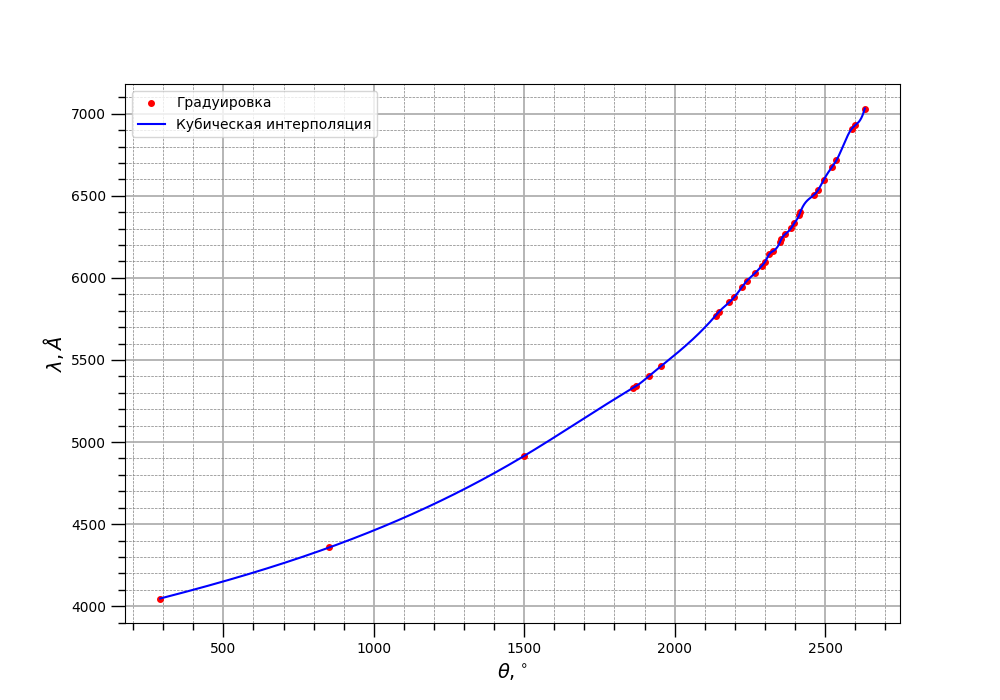
\includegraphics[width=1.1\linewidth]{interpol}
			\caption{Интерполяция полученных данных кубическим сплайном.}
		\end{figure}
	
		\begin{figure}[H]
			\centering
			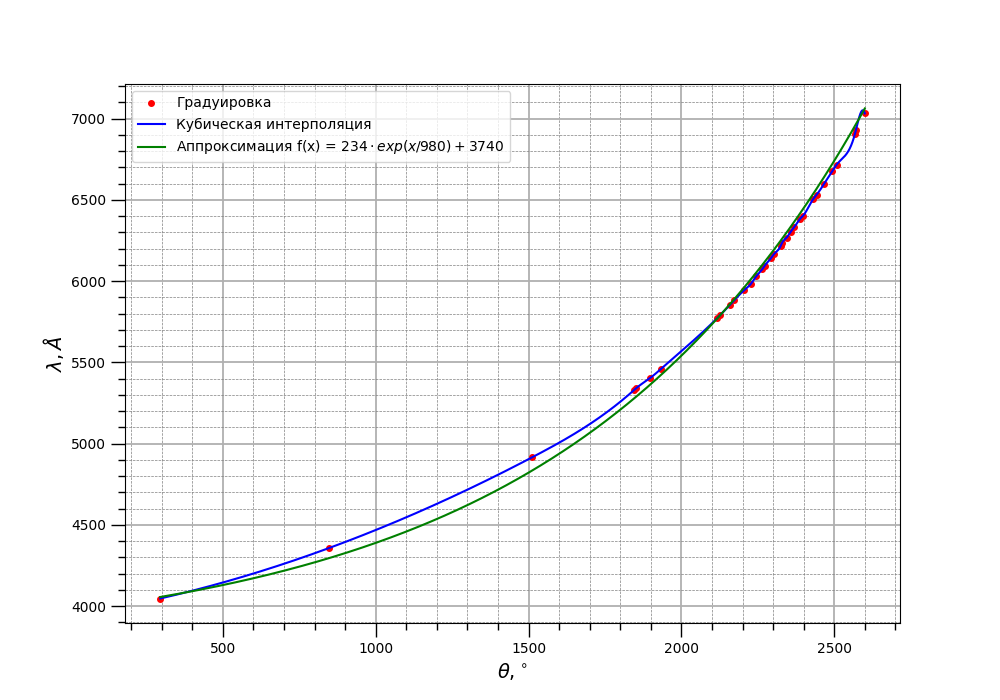
\includegraphics[width=1.1\linewidth]{approx}
			\caption{Аппроксимация полученной функции экспонентой}
		\end{figure}
		
		
		\item Измерим спектр водородной лампы для линий $H_\alpha$, $H_\beta$, $H_\gamma$, $H_\delta$. По градуировочной кривой определим значения длин волн соответствующих спектральных линий. Для каждой наблюдаемой линии определим постоянную Ридберга. Определим ее среднее значение и погрешность. Полученные данные занесем в таблицу 3.
		
		\begin{longtable}{|c|c|c|c|c|}
			\hline
			№ & $H_\alpha$ & $H_\beta$ & $H_\gamma$ & $H_\delta$  \\ \hline
			$\theta, {}^\circ$ & 2482 & 1470 & 822 & 400 \\ \hline
			$\lambda, $ \AA & 6551 $\pm $ 6 & 4883 $\pm $ 2 & 4338 $\pm $ 1 & 4100 $\pm $ 1 \\ \hline
			$R, \cdot 10^7\text{ м}^{-1}$ & 1,0992 $\pm $ 0,0003 & 1,0927 $\pm $ 0,0003& 1,0973 $\pm $ 0,0003& 1,0972 $\pm $ 0,0003\\ \hline
			$\overline{R}, \text{ м}^{-1}$ & \multicolumn{4}{c|}{1,0961 $\pm $ 0,0005}  \\ \hline 
			\caption{Значения угла барабана при различных спектральных линиях водорода. $\sigma_{\theta} = \pm2^\circ$}
		\end{longtable}
	
		Расчет Ридберга проводится по формуле:
			\begin{equation}
				\lambda_{n,m}^{-1} =\frac{m_ee^2}{4\pi\hbar^3c}\left(\frac{1}{m^2}-\frac{1}{n^2}\right) = \text{R} \left(\frac{1}{m^2}-\frac{1}{n^2}\right)
			\end{equation}
		
		 Расчет погрешности  проводился по формулам:
		
		\begin{equation}
			 \sigma_{\overline{R}} = \sqrt{\frac{1}{k(k-1)} \sum_{i = 1}^{k} (\overline{R} - {R_i})^2} = 0,002 \cdot 10^7\text{м}^{-1} 
		\end{equation}
		
		\begin{equation} 
			\sigma_{\overline{R_{\Sigma}}} = \sqrt{ \sigma_{\overline{R}} ^2 + \sigma_{\lambda_{n,m}^{-1}}^2 }, \qquad
			\sigma_{\lambda_{n,m}^{-1}}\cdot R = \sigma_{R} \cdot \lambda
		\end{equation}
	градуировочная кривая аппроксимирована функцией:
	
	\begin{equation}\label{}
		\lambda = 234 \cdot exp (\frac{\theta}{980}) + 3740
	\end{equation}
	Погрешность определения $\lambda$:
	\begin{equation}\label{}
		\sigma_{\lambda} = \frac{234}{980}\cdot exp(\frac{\theta}{980}) \cdot\sigma_{\theta}
	\end{equation}
	
		
		\item Определим деления барабана монохроматора, соответствующие:
		a) линии $h \nu_{1,0}$ - одной нз самых длинноволновых хорошо видимых линий поглощения $\left(n_1, 0\right)$,
		б) линии $h \nu_{1,5}$ - шестой по счету от выбранной длинноволновой линии $\left(h v_{1,5}\right)$,
		в) $h \nu_{\text{гр}}$ - границе схождения спектра (началу сплошного спектра поглощения). По градуировочной кривой определим значения длин волн соответствующих спектральных линий. Полученные данные занесем в таблицу 4.
		
		\begin{longtable}{|c|c|c|c|}
			\hline
			№ & $h \nu_{1,0}$ & $h \nu_{1,5}$ & $h \nu_{\text{гр}}$  \\ \hline
			$\theta, {}^\circ$ & 2404 & 2354 & 1664 \\ \hline
			$\lambda, $ \AA & 6416 $\pm $ 5 & 6234$\pm $ 5 & 5103 $\pm $ 3 \\ \hline
			
			\caption{Значения угла барабана при различных спектральных линиях йода}
		\end{longtable}
		
		
		\item Вычислим энергию колебательного кванта возбужденного состояния молекулы йода.
		
		 $$ h \nu_2 = (h \nu_{1,5} - h \nu_{1,0})/5 = (1,9170 - 1,9732)/5 = 0,01124 \pm  0,00002 \text{ эВ}$$			
		 
		 Погрешность считается по формуле: 
	 	\begin{equation}\label{}
		 	\sigma_{E} = \frac{hc}{\lambda^2} \cdot \sigma_{\lambda}
		 \end{equation}

			
		\begin{figure}[H]
			\centering
			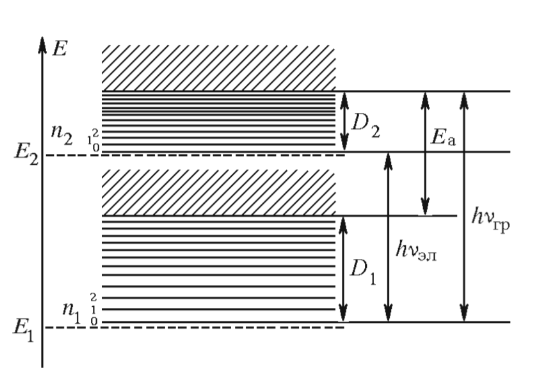
\includegraphics[width=0.6\linewidth]{lev}
			\caption{Электронные и электронно колебательные энергетические уровни двухатомной молекулы}
		\end{figure}
		
		\item По полученным данным и известным значениям энергии колебательно кванта в основном состоянии $h\nu_1 = 0,027$ эВ, энергия возбужденного атома $E_a = 0,94$ эВ, вычислим:
		
		a) энергию электронного перехода $h \nu_{\text{эл}}$,\\
		$$h \nu_{1,0}=h \nu_{\text{эл}}+h\nu_2(0+\dfrac{1}{2})-h \nu_1(1+\dfrac{1}{2})$$
		
		$$ h \nu_{\text{эл}} = 2,086 -  \dfrac{1}{2}\cdot 0,011 + \dfrac{3}{2}\cdot 0,027 = 2,121 \pm  0,003\text{ эВ} $$
		
		б) энергию диссоциации молекулы в основном состоянии Д1;\\
		$$D_1 = h \nu_{\text{гр}} - E_a = 2,410 - 0,940 = 1,470 \pm  0,002\text{ эВ}$$
		
		
		в) энергию диссоциации молекулы в возбужденном состоянии Д2.\\
		$$D_2 = h \nu_{\text{гр}} - h \nu_{\text{эл}} = 2,410 - 2,116 = 0,294 \pm  0,005\text{ эВ}$$
		
		
		
		
		\textbf{Обсуждение результатов и выводы: }\\
		
		В ходе данной работы мы исследовали сериальные закономерности в оптическом спектре водорода. Также исследовали поглощения паров йода в видимой области. Построили градуировочную кривую спектрометра по измерениям спектра неона и ртути.\\
		По результатам измерений мы определили константу Ридберга $\overline{R} = 1,0961 \pm 0,0005\cdot 10^7\text{ м}^{-1}$. В пределах погрешности значение не совпадает с теоретическим $ R = 1,0973\cdot 10^7\text{ м}^{-1}$, хотя находится достаточно близко.\\
		Получили энергию колебательного кванта возбужденного состояния молекулы йода $ h \nu_2 = 0,01124 \pm 0,00002 \text{ эВ}$, энергию электронного перехода  $h \nu_{\text{эл}} = 2,121 \pm 0,003 \text{ эВ}$ и энергии диссоциации молекулы в основном $D_1 = 1,470 \pm 0,002\text{ эВ}$ и в возбужденном состоянии $D_2 = 0,294 \pm 0,005\text{ эВ}$.
		
		Используемый нами спектрометр позволяет получать значения длин волн с достаточно большой точностью, поэтому дальнейшие расчеты, использующие градуировочную кривую также имеют высокую точность. Соответственно, последующие расчеты хорошо согласуются с теоретическими оценками. 
		
	
	
	
		

		
	\end{enumerate}
	\end{document}